\section{Objective}
\label{sec:7-1}

Measure how well each model assigns sentiment to reviews it has not seen, compare the two networks fairly, and find where they fail. The protocol is fixed before the results: Macro-F1 (Section~\ref{sec:2-4}) is the main metric; the test part of 39{,}358 reviews is read once; every choice (epoch, neutral threshold) is made on the validation part. Confidence intervals come from 1{,}000 bootstrap resamples of the test reviews, with all models scored on the same resample so that differences can be paired. The intervals reflect the sampling error of the test part only, not the choice of random seed.

\section{Results on the Full Test Part}
\label{sec:7-2}

\begin{center}
\small
\begin{tabular}{@{}lrrrrrr@{}}
    \toprule
    Model & Accuracy & Macro-F1 & \shortstack[r]{F1\\negative} & \shortstack[r]{F1\\neutral} & \shortstack[r]{F1\\positive} & \shortstack[r]{Macro-F1\\95\% interval} \\
    \midrule
    BERT-base fine-tuned & \textbf{0.9074} & \textbf{0.7877} & \textbf{0.8470} & \textbf{0.5540} & \textbf{0.9620} & [0.7814, 0.7929] \\
    BiLSTM + attention & 0.8788 & 0.7422 & 0.7863 & 0.4916 & 0.9488 & [0.7360, 0.7480] \\
    Always positive & 0.7794 & 0.2920 & 0 & 0 & 0.8760 & [0.2911, 0.2929] \\
    \bottomrule
\end{tabular}
\end{center}

\begin{center}
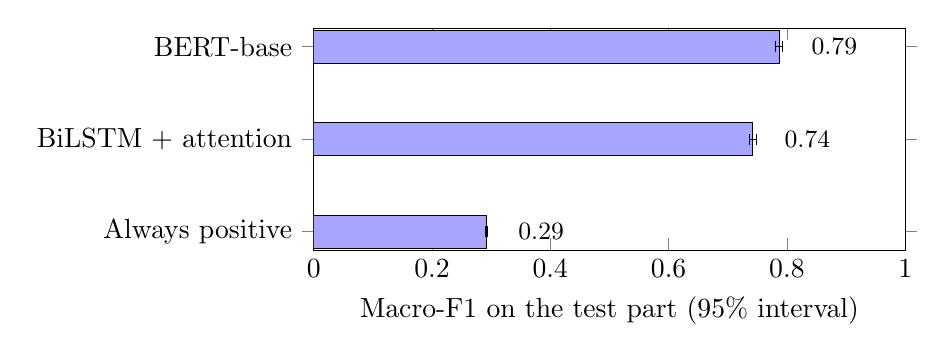
\begin{tikzpicture}
\begin{axis}[
  xbar, xmin=0, xmax=1, width=0.75\textwidth, height=4.4cm,
  symbolic y coords={Always positive,BiLSTM + attention,BERT-base},
  ytick=data, xlabel={Macro-F1 on the test part (95\% interval)},
  bar width=12pt, nodes near coords, nodes near coords align={horizontal},
  every node near coord/.append style={font=\small, xshift=8pt}
]
\addplot[fill=blue!35, error bars/.cd, x dir=both, x explicit] coordinates {
  (0.2920,Always positive) += (0.0009,0) -= (0.0009,0)
  (0.7422,BiLSTM + attention) += (0.0058,0) -= (0.0062,0)
  (0.7877,BERT-base) += (0.0052,0) -= (0.0063,0)
};
\end{axis}
\end{tikzpicture}
\end{center}

Both networks are far above the always-positive rule (Macro-F1 0.292, which scores 0.78 accuracy while recognising nothing about the other two classes). BERT is best on every column. The F1 of the neutral class is the lowest for both networks, 0.49 and 0.55.

\textbf{Cost.} Both networks were trained and timed on a Tesla T4.

\begin{center}
\small
\begin{tabular}{@{}lrrr@{}}
    \toprule
    Model & Training time & Inference on the test part & Parameters \\
    \midrule
    BERT-base & 64.4 min & 83.7 s & 109.48 M \\
    BiLSTM + attention & 3.4 min & 3.7 s & 6.25 M \\
    \bottomrule
\end{tabular}
\end{center}

BERT needs about 19 times the training time, 23 times the inference time and 17.5 times the parameters of the BiLSTM for 0.0455 more Macro-F1. The BiLSTM reaches about 94\% of the Macro-F1 of BERT with about 5\% of its training time.

\section{Is the Neutral Class the Problem?}
\label{sec:7-3}

Both networks have high recall but low precision on neutral: they predict neutral for too many reviews. The table gives, for each model, the share of true neutral reviews that are predicted correctly, and the true label of the reviews it predicts as neutral.

\begin{center}
\small
\begin{tabular}{@{}lrrrrrr@{}}
    \toprule
     & \multicolumn{3}{c}{True neutral predicted as} & \multicolumn{3}{c}{Predicted neutral are truly} \\
    \cmidrule(lr){2-4}\cmidrule(lr){5-7}
    Model & negative & neutral & positive & negative & neutral & positive \\
    \midrule
    BERT-base & 19.7\% & 68.1\% & 12.1\% & 17.9\% & 46.7\% & 35.4\% \\
    BiLSTM + attention & 16.5\% & 67.6\% & 15.9\% & 23.4\% & 38.6\% & 38.0\% \\
    \bottomrule
\end{tabular}
\end{center}

Both networks recover about two thirds of the neutral reviews, but fewer than half of the reviews they call neutral are neutral. The cause is partly the data (a 3-star review often praises and complains at once, and the neutral class has no vocabulary of its own, Section~\ref{sec:4-8}) and partly the loss, whose neutral weight is 4.4 times a typical weight (Section~\ref{sec:5-7}).

\section{Performance by Review Length}
\label{sec:7-5}

\begin{center}
\small
\begin{tabular}{@{}lrrrrrr@{}}
    \toprule
    Words per review & $\le$30 & 31--60 & 61--100 & 101--200 & 201--400 & $>$400 \\
    Reviews in the test part & 6{,}137 & 13{,}659 & 9{,}601 & 7{,}534 & 2{,}100 & 327 \\
    \midrule
    BERT-base & 0.778 & 0.783 & 0.794 & 0.796 & 0.758 & 0.693 \\
    BiLSTM + attention & 0.753 & 0.738 & 0.746 & 0.747 & 0.704 & 0.600 \\
    \bottomrule
\end{tabular}
\end{center}

Both models are lowest on reviews longer than 400 words, and the BiLSTM drops the most (0.600 against 0.693 for BERT). The BiLSTM keeps only the first 200 words and BERT the first 256 tokens, so both lose the end of a long review. The last group has only 327 reviews, so its scores vary more and should not be over-read.

\section{Bootstrap Interval for the Difference}
\label{sec:7-6}

The difference in Macro-F1 between BERT and the BiLSTM on the full test part is $+0.0454$, with a 95\% interval of $[+0.0400,\,+0.0507]$ over the paired bootstrap resamples. The interval does not contain zero, so the difference is larger than the sampling error of the test part, and BERT is ahead of the BiLSTM in 100\% of the resamples.

\section{Calibrating the Neutral Threshold}
\label{sec:7-7}

Because the models over-predict neutral, a constant \texttt{bias} is added to the log-probability of neutral before taking the arg\,max (a negative bias predicts neutral less often). The bias is chosen on the validation part to maximise Macro-F1 and then applied once to the test part. This needs no retraining.

\begin{center}
\small
\begin{tabular}{@{}lrrrr@{}}
    \toprule
    Model & \shortstack[r]{Chosen\\bias} & \shortstack[r]{Validation Macro-F1\\before $\to$ after} & \shortstack[r]{Test Macro-F1\\before $\to$ after} & \shortstack[r]{Test F1 neutral\\before $\to$ after} \\
    \midrule
    BiLSTM + attention & $-0.8$ & 0.7504 $\to$ 0.7577 & 0.7422 $\to$ 0.7551 & 0.4916 $\to$ 0.4978 \\
    BERT-base & $-1.1$ & 0.7864 $\to$ 0.7902 & 0.7877 $\to$ 0.7866 & 0.5540 $\to$ 0.5448 \\
    \bottomrule
\end{tabular}
\end{center}

The adjustment helps the BiLSTM (+0.013 on the test part) but not BERT: the gain of 0.004 that BERT shows on validation does not carry over to the test part and lies within the noise. The headline results of this report use no bias (Section~\ref{sec:7-2}); the calibration is an extra experiment.

\section{Error Analysis and Examples}
\label{sec:7-8}

\subsection*{Confident errors of the best model}

BERT predicts \emph{negative} for 165 reviews of 5 stars and \emph{positive} for 58 reviews of 1 star; 948 neutral reviews are misclassified. Many confident errors look like noisy labels: the author gave 5 stars but wrote a complaint (``Now I would not recommend it to my worst enemy. The coffee now has no aroma\ldots'', ``Incredibly overpriced\ldots this is a total and complete rip off''), or 1 star with praise (``LOVE LOVE LOVE THESE! (edited because NO longer available in prime)''). In these cases the model reads the text better than the star count does. Not every case is noise: ``My dogs won't eat anything else. My dogs will not eat anything but the Iams biscuit'' praises the product, and the model misreads it. The share of noisy labels among the errors was not counted, so this report does not give a rate.

A related property of the data: about 3.4\% of test reviews (1{,}350) contain a phrase such as ``3 stars'', and only about 59\% of them state the true rating (the others read ``5 star service'' or ``4 stars out of 5''). These texts are kept, so some signal flows from the label into the text for both models.

\subsection*{Sentences written for the test}

Six sentences written by the authors give a qualitative check; they are not a substitute for the measurements above.

\begin{center}
\small
\begin{tabular}{@{}p{7.2cm}ll@{}}
    \toprule
    Sentence & BiLSTM & BERT \\
    \midrule
    ``This coffee is absolutely amazing, I will definitely buy it again!'' & pos (100\%) & pos (100\%) \\
    ``Not bad at all, actually pretty tasty.'' & neu (78\%) & pos (79\%) \\
    ``It's okay. Nothing special, but it does the job.'' & neu (100\%) & neu (99\%) \\
    ``Great, another box arrived completely crushed. Just what I needed.'' & pos (87\%) & pos (99\%) \\
    ``My dog loves these treats, but they are way too expensive for such a small bag.'' & neu (84\%) & neu (89\%) \\
    ``I would not recommend this to anyone. Total waste of money.'' & neg (100\%) & neg (100\%) \\
    \bottomrule
\end{tabular}
\end{center}

Both models read the sarcastic fourth sentence as positive, because ``great'' and ``just what I needed'' sound positive. Both label the mixed third and fifth sentences neutral, and the clearly positive and negative sentences correctly. For the second sentence the BiLSTM answers neutral and BERT positive; both are acceptable for such mild praise. The attention weights of the BiLSTM mostly fall on words that carry sentiment or reverse it (\emph{mistake}, \emph{great}, \emph{not}, \emph{okay}, \emph{but}), but not always: for one neutral review the largest weight is on a product name (\emph{stevia}). Attention shows where the model looks, not a complete explanation.

\section{Limitations}
\label{sec:7-9}

\begin{itemize}
    \item \textbf{Weak labels.} Stars do not always match the text (Section~\ref{sec:7-8}), and the 3-star boundary is subjective, which bounds the quality any model can show.
    \item \textbf{Sarcasm and mixed opinions.} Both models fail on sarcasm, and neutral stays the hardest class (F1 0.49 and 0.55).
    \item \textbf{Random split.} The label distribution drifts over time (Section~\ref{sec:4-5}) and the same user or product can sit in both training and test, so the scores do not measure performance on future reviews.
    \item \textbf{Runs and seeds.} Each model was trained once (seed 42), so the bootstrap intervals do not cover variation between seeds.
    \item \textbf{BERT is not saturated.} It was fine-tuned for 2 epochs with one fixed configuration, so its score may be a lower bound.
    \item \textbf{Different truncation.} The BiLSTM keeps 200 words and BERT 256 tokens.
    \item \textbf{One domain.} All data are English food reviews from Amazon, 1999--2012.
\end{itemize}
